\chapter{Future Work and Improvements}

\section{Limitations of the Current Version}

While our current version provides a solid foundation for modeling and simulating various physical systems, it has several limitations that need to be addressed:

\begin{itemize}
    \item \textbf{Limited Physics Models:} The current version only supports basic physics models such as particle systems and rigid bodies. More advanced physics phenomena such as rotational dynamics, fluid flow, soft body deformation, and electrical circuits are not yet implemented.
    \item \textbf{Simplified Interaction:} Interaction with simulated objects is limited to basic controls such as start, stop, and reset. More interactive features such as user-defined forces and constraints are missing.
    \item \textbf{Performance Constraints:} As simulations become more complex and include a larger number of objects, the performance of the application may degrade. Optimization techniques are needed to improve performance and scalability.
\end{itemize}

Addressing these limitations will enhance the capabilities and usability of our simulation tool.

\section{Potential Enhancements and Features to be Added}

To improve the functionality and usability of the simulation tool, the following enhancements and features can be added:

\begin{itemize}
    \item \textbf{Advanced Physics Models:} Implement support for rotational dynamics, fluid simulation, soft body simulation, and electrical simulation to cover a wider range of physical phenomena.
    \item \textbf{Enhanced User Interaction:} Introduce more interactive features such as drag-and-drop object placement, user-defined forces and constraints, and real-time parameter adjustments.
    \item \textbf{Simulation Control:} Provide finer control over simulations, including the ability to pause and resume simulations, adjust simulation speed, and save and load simulation states.
    \item \textbf{Visualization Improvements:} Enhance the 3D visualization capabilities with better rendering techniques, support for textures and materials, and improved lighting and shading effects.
\end{itemize}

These enhancements will make the simulation tool more versatile and user-friendly, catering to a broader range of users and applications.

\section{Long-term Vision for the Project}

Our long-term vision for the project is to create a comprehensive and versatile simulation platform that can be used for a wide range of applications. This includes:

\begin{itemize}
    \item \textbf{Rotational Systems:} Implement support for simulating rotational dynamics, including rigid body rotation, torque, angular momentum, and rotational collisions.
    
    \begin{center}
    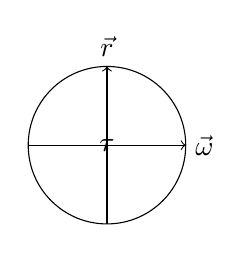
\begin{tikzpicture}
        % Draw rotational system diagram
        \draw (0,0) circle (1);
        \draw[->] (-1,0) -- (1,0) node[right] {$\vec{\omega}$};
        \draw[->] (0,-1) -- (0,1) node[above] {$\vec{r}$};
        \node at (0,0) {$\tau$};
    \end{tikzpicture}
    \end{center}
    
    \item \textbf{Fluid Simulation:} Develop algorithms for simulating fluid flow, including fluid dynamics, viscosity, turbulence, and buoyancy effects.
    
    \item \textbf{Soft Body Simulation:} Implement methods for simulating deformable objects such as cloth, rubber, and biological tissues, with support for elasticity, damping, and collisions.
    
    \item \textbf{Electrical Simulation:} Model electrical circuits and components such as resistors, capacitors, and inductors, and simulate electrical behavior including voltage, current, and power.
\end{itemize}

By incorporating these advanced features and expanding the capabilities of the simulation platform, we aim to provide researchers, engineers, educators, and hobbyists with a powerful tool for exploring and understanding the physical world.
